% Created 2018-03-05 Mon 19:26
\documentclass{article}
\usepackage[mathletters]{ucs}
\usepackage[utf8x]{inputenc}
\usepackage[T1]{fontenc}
\usepackage{fixltx2e}
\usepackage{graphicx}
\usepackage{longtable}
\usepackage{float}
\usepackage{wrapfig}
\usepackage{rotating}
\usepackage[normalem]{ulem}
\usepackage{amsmath}
\usepackage{textcomp}
\usepackage{marvosym}
\usepackage{wasysym}
\usepackage{amssymb}
\usepackage{hyperref}
\tolerance=1000
\date{\today}
\title{Notebook1}
\hypersetup{
  pdfkeywords={},
  pdfsubject={},
  pdfcreator={Emacs 25.3.1 (Org mode 8.2.10)}}
\begin{document}

\maketitle
\tableofcontents

\section{Mathematical Description of the Discrete Cosine Transform}
\label{sec-1}
\begin{enumerate}
\item Brief Overview
\label{sec-1-1}
\begin{itemize}
\item The Discrete cosine transform can represent an image as a sum of
sinusoids with frequencies and magnitudes that differ.
\item The Cosine transform has the property that most of the important
bits of information with an image (or even an audio wave) is
concentrated (Notebook 2 will expand on this idea).
\item Due to this property, the DCT (or the Modified discrete cosine transofrm)
is used to MP3 compression and for JPG compression.
\end{itemize}
\item The Equation
\label{sec-1-2}
\begin{itemize}
\item The Two dimensional DCT of an M-by-N matrix can be expressed as
follows. \\
  C$_{\text{pq}}$ = α$_{\text{p}}$α$_{\text{q}}$ $\sum^{M-n}_{m = 0}\sum^{N-1}_{n = 0} A_{mn}\cos\frac{π(2m + 1)p}{2M}\cos\frac{π(2n + 1)q}{2N}$
\\ $\quad{}$ where
\\ $\quad{} \quad{}$ 0 ≤ p ≤ M - 1
\\ $\quad{} \quad{}$ 0 ≤ q ≤ N - 1
\\ $\quad{} \quad{}$ α$_{\text{p}}$ = $\begin{cases} 1/\sqrt{M} & p = 0 \\
                                            \sqrt{2/M} & 1 ≤ p ≤ M-1
                               \end{cases}$
\\ $\quad{} \quad{}$ α$_{\text{q}}$ = $\begin{cases} 1/\sqrt{N} & p = 0 \\
                                            \sqrt{2/N} & 1 ≤ q ≤ N-1
                               \end{cases}$
\item We can note that if we assign p = n and q = n, they both fit the domain of p and q, and I will be using this for the program
\end{itemize}
\end{enumerate}
\section{Implementation and Graphing of the Discrete Cosine Transform}
\label{sec-2}
\begin{itemize}
\item So first we must implement the mathematical equation above
\begin{itemize}
\item The following code can be found in Cosine.hs
\begin{verbatim}
import Data.List.Split

dcBasis :: (Floating p1, Eq p1) => p1 -> p1 -> Int -> Int -> [[p1]]
dcBasis p q m n = chunksOf n $ (*) . (αpq *) <$> ti <*> tj
  where compAlpha x bound
          | x == 0    = 1 / sqrt bound
          | otherwise = sqrt (2 / bound)
        mfloat           = fromIntegral m
        nfloat           = fromIntegral n
        αpq              = compAlpha p mfloat * compAlpha q nfloat
        f offset bound x = cos $ (pi * offset * (2 * x + 1)) / (2 * bound) -- x is
        ti               = f p mfloat . fromIntegral <$> [0..(n-1)] -- an element
        tj               = f q nfloat . fromIntegral <$> [0..(m-1)] -- of a vector
\end{verbatim}
\begin{itemize}
\item Lets break down this function line by line, the first
function is \texttt{compAlpha} which basically abstracts out the logic
for α$_{\text{p}}$ and α$_{\text{q}}$ seen in the mathematical equation, we can see the
application of this in \texttt{apq} which just multiplies a$_{\text{p}}$ by a$_{\text{q}}$
basically. As described in the math we just set p and q to m and n
respectively.

\item \texttt{mfloat} and \texttt{nfloat} basically just turn m and n into a float
respectively.

\item \texttt{f} is once again another abstraction that abstracts out the
$\cos\frac{π(2m + 1)p}{2M}$ and the n variant seen in the
mathematics.

\item thus \texttt{ti} and \texttt{tj} computes this abstraction for all values from 0
to N-1 for the one dealing with n's (while also giving the
correct p value) and 0 to M-1 for the one dealing with m's (while
also giving the correct q value).

\item Now all we have to do is combine our computations which comes in
\texttt{chunksOf n \$ (*) . (αpq *) <\$> ti <*> tj}. \\
      the \texttt{(*) . (αpq *)} is really a function that takes 2 numbers
before becoming a value so, \texttt{(*) . (αpq *) <\$> ti} has the type
signature [Num a ⇒ a → a] (as \texttt{<\$>} is just map). Now, \texttt{<*>} we
can think of as the generalized cross product in which the order
can be seen in the example below. Noting this, we can now notice
that the nested summation in reality for creating indices is
exactly the same as using the applicative (\texttt{<*>}) with the
function containg the m points and the right argument containg the
n points for the computation of a nxm long matrix. The final
part of \texttt{chunmksOf n} simply just formats the data into a list
that is really nxm instead of flat
\begin{itemize}
\item \texttt{[(1 +), (-) 99] <*> [1,2,3] ≡ [2,3,4,98,97,96]}
\end{itemize}
\end{itemize}
\end{itemize}
\item Now that we have the formula up, we can now easily create any nxn
matrix asked (the prompt asks for 16x16, but I'll make it generic)
\begin{verbatim}
nbyN :: (Floating a, Eq a, Enum a) => Int -> [[[[a]]]]
nbyN n = chunksOf n $ (\x y -> dcBasis x y n n) <$> [0..(fromIntegral n-1)]
                                                <*> [0..(fromIntegral n-1)]
eightByEight :: [[[[Double]]]]
eightByEight = nbyN 8
\end{verbatim}
\begin{itemize}
\item here we create the NxN matrix by simply calling dcBasis with all
permutations of x and y, we do this by applying the same trick as
above (refer to the above explanation for the \texttt{f <\$>} x$_{\text{1}}$ \texttt{<*>}
x$_{\text{2}}$ pattern).
\item Notice that our structure is not a 2d vector instead a 2d list
containing 2d lists.
\end{itemize}
\item Now that we have the data, we must normalize it, because if we look
at the last row in the last 2d list, we see their values really are
too small to effectively Grey scale them.
\begin{itemize}
\item \texttt{eightByEight !! 7 !! 7 !! 7} ≡ [-9.515058436089173e-3,2.7096593915592444e-2,-4.055291860268229e-2,4.7835429045636306e-2,-4.78354290456363e-2,4.055291860268227e-2,-2.7096593915592413e-2,9.515058436089185e-3]

\item so in the file \texttt{Normalize.hs} Ι make a normalization type and a
function to compute such a type
\begin{verbatim}
import Misc
-- Really only going to use ZeroC for now, but can expand later
data Normalize = Zeroc
               | Same


normalizeValues :: (Functor f1, Fractional b, Foldable f1, Ord b) => Normalize -> f1 [b] -> f1 [b]
normalizeValues Same  xss = undefined
normalizeValues Zeroc xss = (/ greatest) <$$> xss
  where flattened = concat xss
        greatest  = maximum (abs <$> flattened)
\end{verbatim}
\begin{itemize}
\item so I only have two cases for the Normalize type, either it's
normalized at zero or it's the same everywhere, for simplicity
Ι only defined the normalizeValues for centering at zero. It's
a really simple formula, I just do element wise division (\texttt{<\$\$>}
is a helper function that just composes 2 maps so I can get the
elements in a doubly nested structure) from the greatest value
after taking the absolute value.

\item Notice that this only works on a 2d list, and not our 4d list, we'll
see how I handle this in the next section
\end{itemize}
\end{itemize}
\item Finally we are ready to plot our Cosine transform, it took me a
while to actually make this as Ι had to search for the correct
plotting function.
\begin{verbatim}
-- the fmap ((-1) :) . (<> [-1]) is for padding the top and bottom
-- this pads the left and right (padList <>) . (<> padList)
plotDCT :: Int -> IO ()
plotDCT n = imshow (fromBlocks (fromLists <$$> padded))
  where padded  = fmap (((-1) :) . (<> [-1])) . (padList <>) . (<> padList) <$$> norm
        padList = [replicate n (-1)]
        norm    = normalizeValues Zeroc <$$> nbyN n -- name shortened for pdf
\end{verbatim}
\begin{itemize}
\item Here we create norm, which is just the normalized vector, we
double map through the 4d list so we can treat each section as a
2d list
\item from here Ι pad the list by double mapping this norm by the
strategy described in the comments.
\item Now I double map into this padded array to turn each section into
a matrix with the double type, and then the fromBlocks function
handles converting the doubly nested list of matricies into a
single matrix which finally allows imshow to graph it.
\item Note that this algorithm can take an \texttt{n}, so we can map any NxN
discrete matrix
\end{itemize}
\item Time to show off the graphs! Note that white on other people's
versions is black here
\begin{itemize}
\item \includegraphics[width=.9\linewidth]{/home/loli/Documents/Workspace/Haskell/Class/531/eecs531-jxo136/Assignment2/data/CosineGraph4x4.png}

\begin{itemize}
\item So this one here is the 4x4 Discrete Cosine Transform, really
this one is quite low res and thus doesn't carry too much detail,
but we can see the checker board shape starting to emerge on the
bottom right
\end{itemize}

\item \includegraphics[width=.9\linewidth]{/home/loli/Documents/Workspace/Haskell/Class/531/eecs531-jxo136/Assignment2/data/CosineGraph.png}
\begin{itemize}
\item This is the 8x8 Discrete Matrix Cosine Transform, notice that 4,4
is the most clear. This pattern will come up in the rest.
\end{itemize}

\item \includegraphics[width=.9\linewidth]{/home/loli/Documents/Workspace/Haskell/Class/531/eecs531-jxo136/Assignment2/data/CosineGraph16x16-full.png}

\begin{itemize}
\item This is the 16x16 which was requested by the assignment, as can
be seen, as you go right and down the checker board gets more and
more fine. Also notice that the 8,8 one is the most clear
matrix, and that on the top row and left column, there are only
vertical and horizontal lines respectively
\end{itemize}
\item \includegraphics[width=.9\linewidth]{/home/loli/Documents/Workspace/Haskell/Class/531/eecs531-jxo136/Assignment2/data/CosineGraph20x20-full.png}
\item 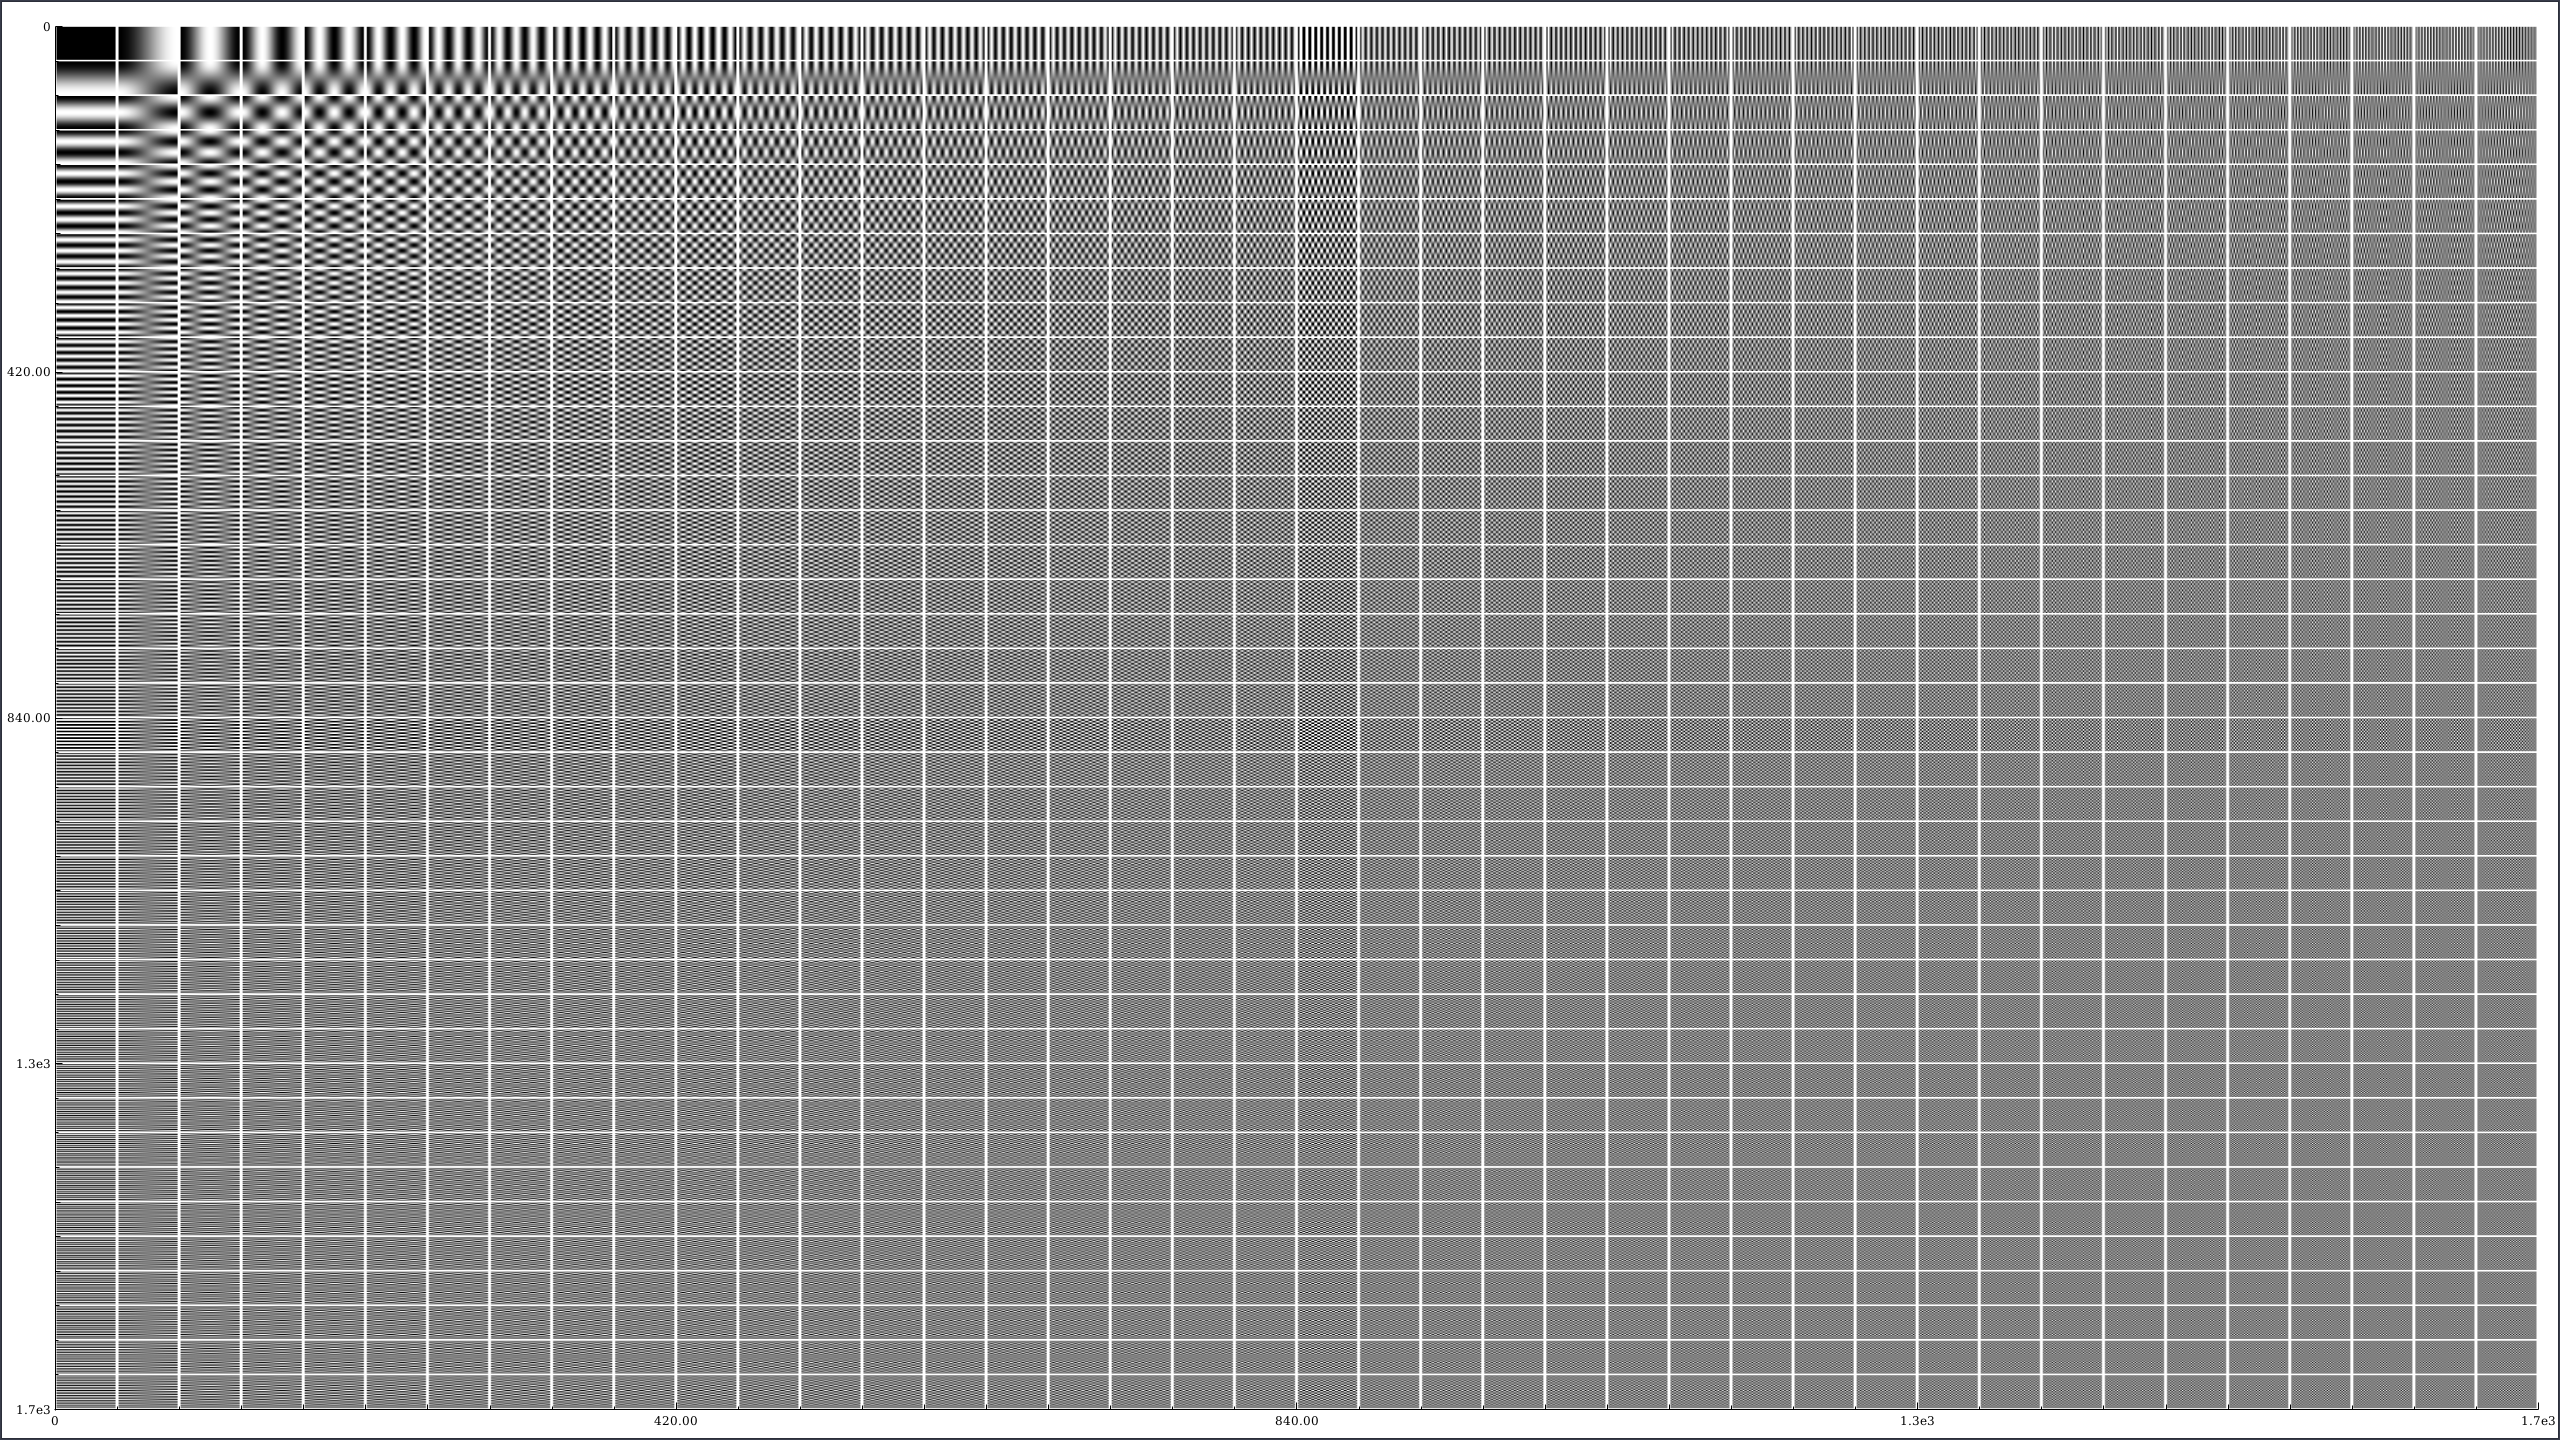
\includegraphics[width=.9\linewidth]{/home/loli/Documents/Workspace/Haskell/Class/531/eecs531-jxo136/Assignment2/data/CosineGraph40x40-full.png}
\begin{itemize}
\item I also plotted the 40x40 and the 20x20 for fun, it might be hard
to see in the pdf, but the 20,20 and the 10,10 transforms are the
most clear
\end{itemize}
\end{itemize}
\end{itemize}
% Emacs 25.3.1 (Org mode 8.2.10)
\end{document}